\paragraph{Recupero password}

\label{Recupero password}

\begin{figure}[ht]
	\centering
	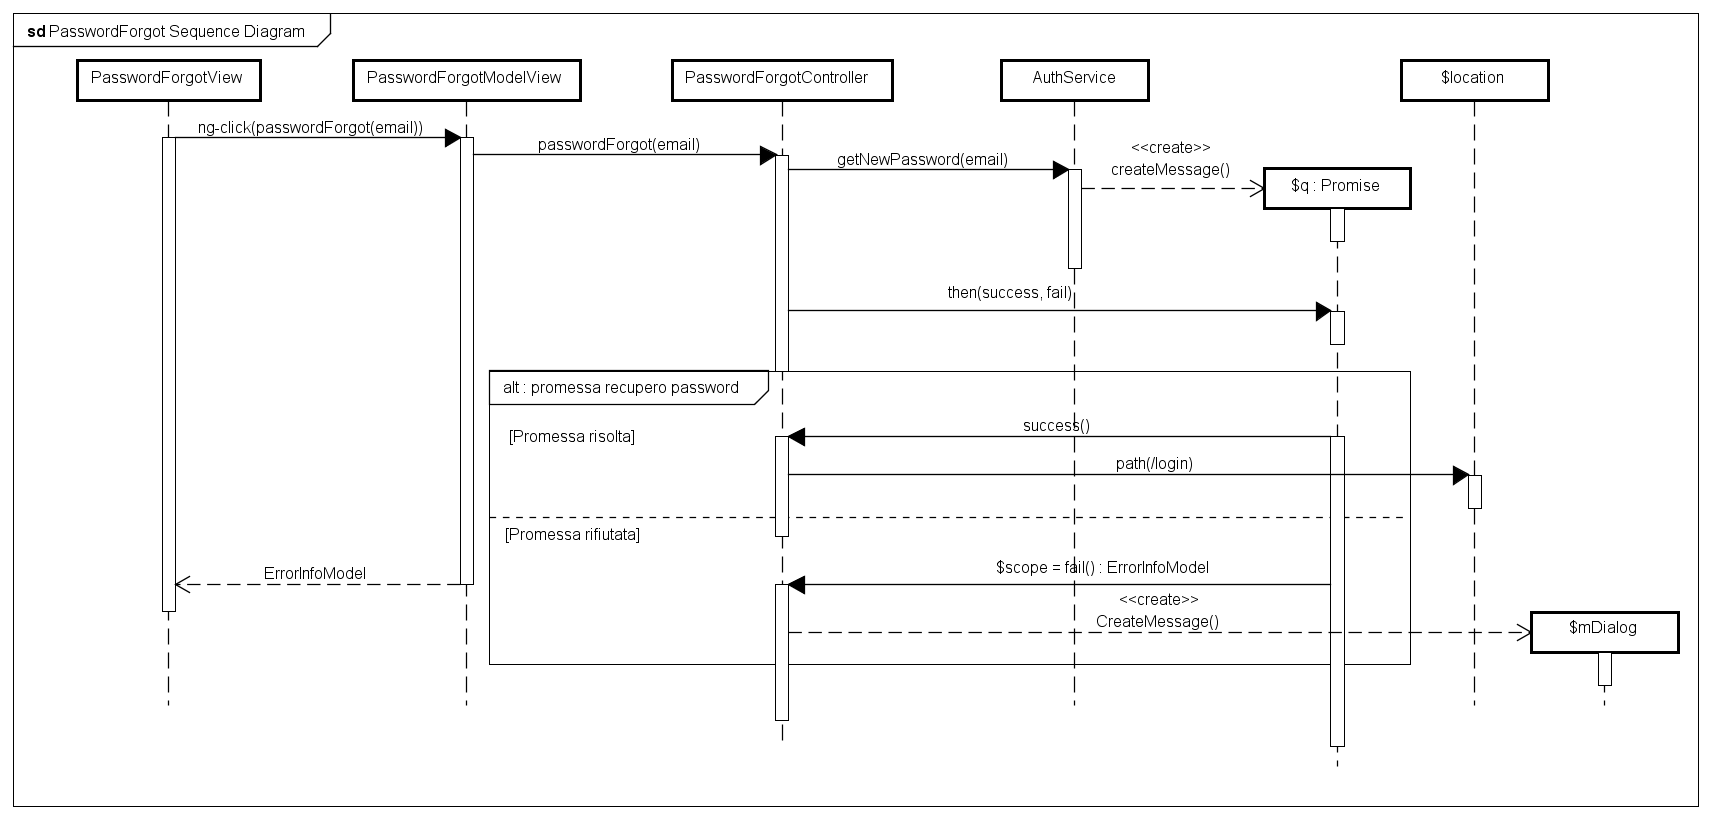
\includegraphics[scale=0.35,keepaspectratio]{UML/DiagrammiDiSequenza/Front-end/PasswordForgot.png}
	\caption{Recupero password}
\end{figure} \FloatBarrier

L'utente, dopo aver inserito la propria email, può recuperare una nuova password avviando l'evento associato al bottone presente in \texttt{PasswordForgotView}. Il \texttt{PasswordForgotController} gestisce l'evento chiamando il metodo \texttt{getNewPassword} dell'\texttt{AuthService}, il quale restituirà una promessa. Se la promessa viene soddisfatta allora verrà mandata una email con la nuova password e verrà reindirizzato alla pagina di login, altrimenti verrà restituito un oggetto di tipo \texttt{ErrorInfoModel} e mostrato a video mediante \texttt{\$mdDialog}. 